\section{Ablations in depth}
\label{sec:ablations}

An \emph{ablation} changes exactly one design choice and re-runs the identical evaluation, so any
change in the score is attributable to that one choice (\emph{ceteris paribus}). Unless noted, the
single-knob ablations are on \vggt/7-Scenes and scored by \ause\ (lower is better; recall from
\Cref{sec:primer-metrics} that \ause\ is rank-only, so calibration cannot move it---calibration is
scored by \ece). Every number is read directly from the result CSVs. \Cref{tab:ablfull} and
\Cref{fig:ablgrid} give the full A1--A12 sweep; we then discuss the two design-defining knobs in
depth, summarize the rest, and finish with the calibration (\Cref{sec:abl-calib}) and fusion
(\Cref{sec:abl-fusion}) studies.

\begin{table*}[t]
\centering\small
\adjustbox{max width=\textwidth}{\input{tables/tab_ablation_full}}
\caption{Full single-knob ablation A1--A12 (\vggt/7-Scenes; \ause\dn\ except A8, which is \ece\dn).
\best{Bold} marks the best level per factor. Alignment (A7) is the dominant knob
($0.715\!\to\!0.496$); calibration (A8) moves only \ece\ ($0.296\!\to\!0.094$, $\sim 3\times$);
held-out fusion weights (A12) $\approx$ equal ($0.585$ vs.\ $0.586$).}
\label{tab:ablfull}
\end{table*}

\begin{figure*}[t]
  \centering
  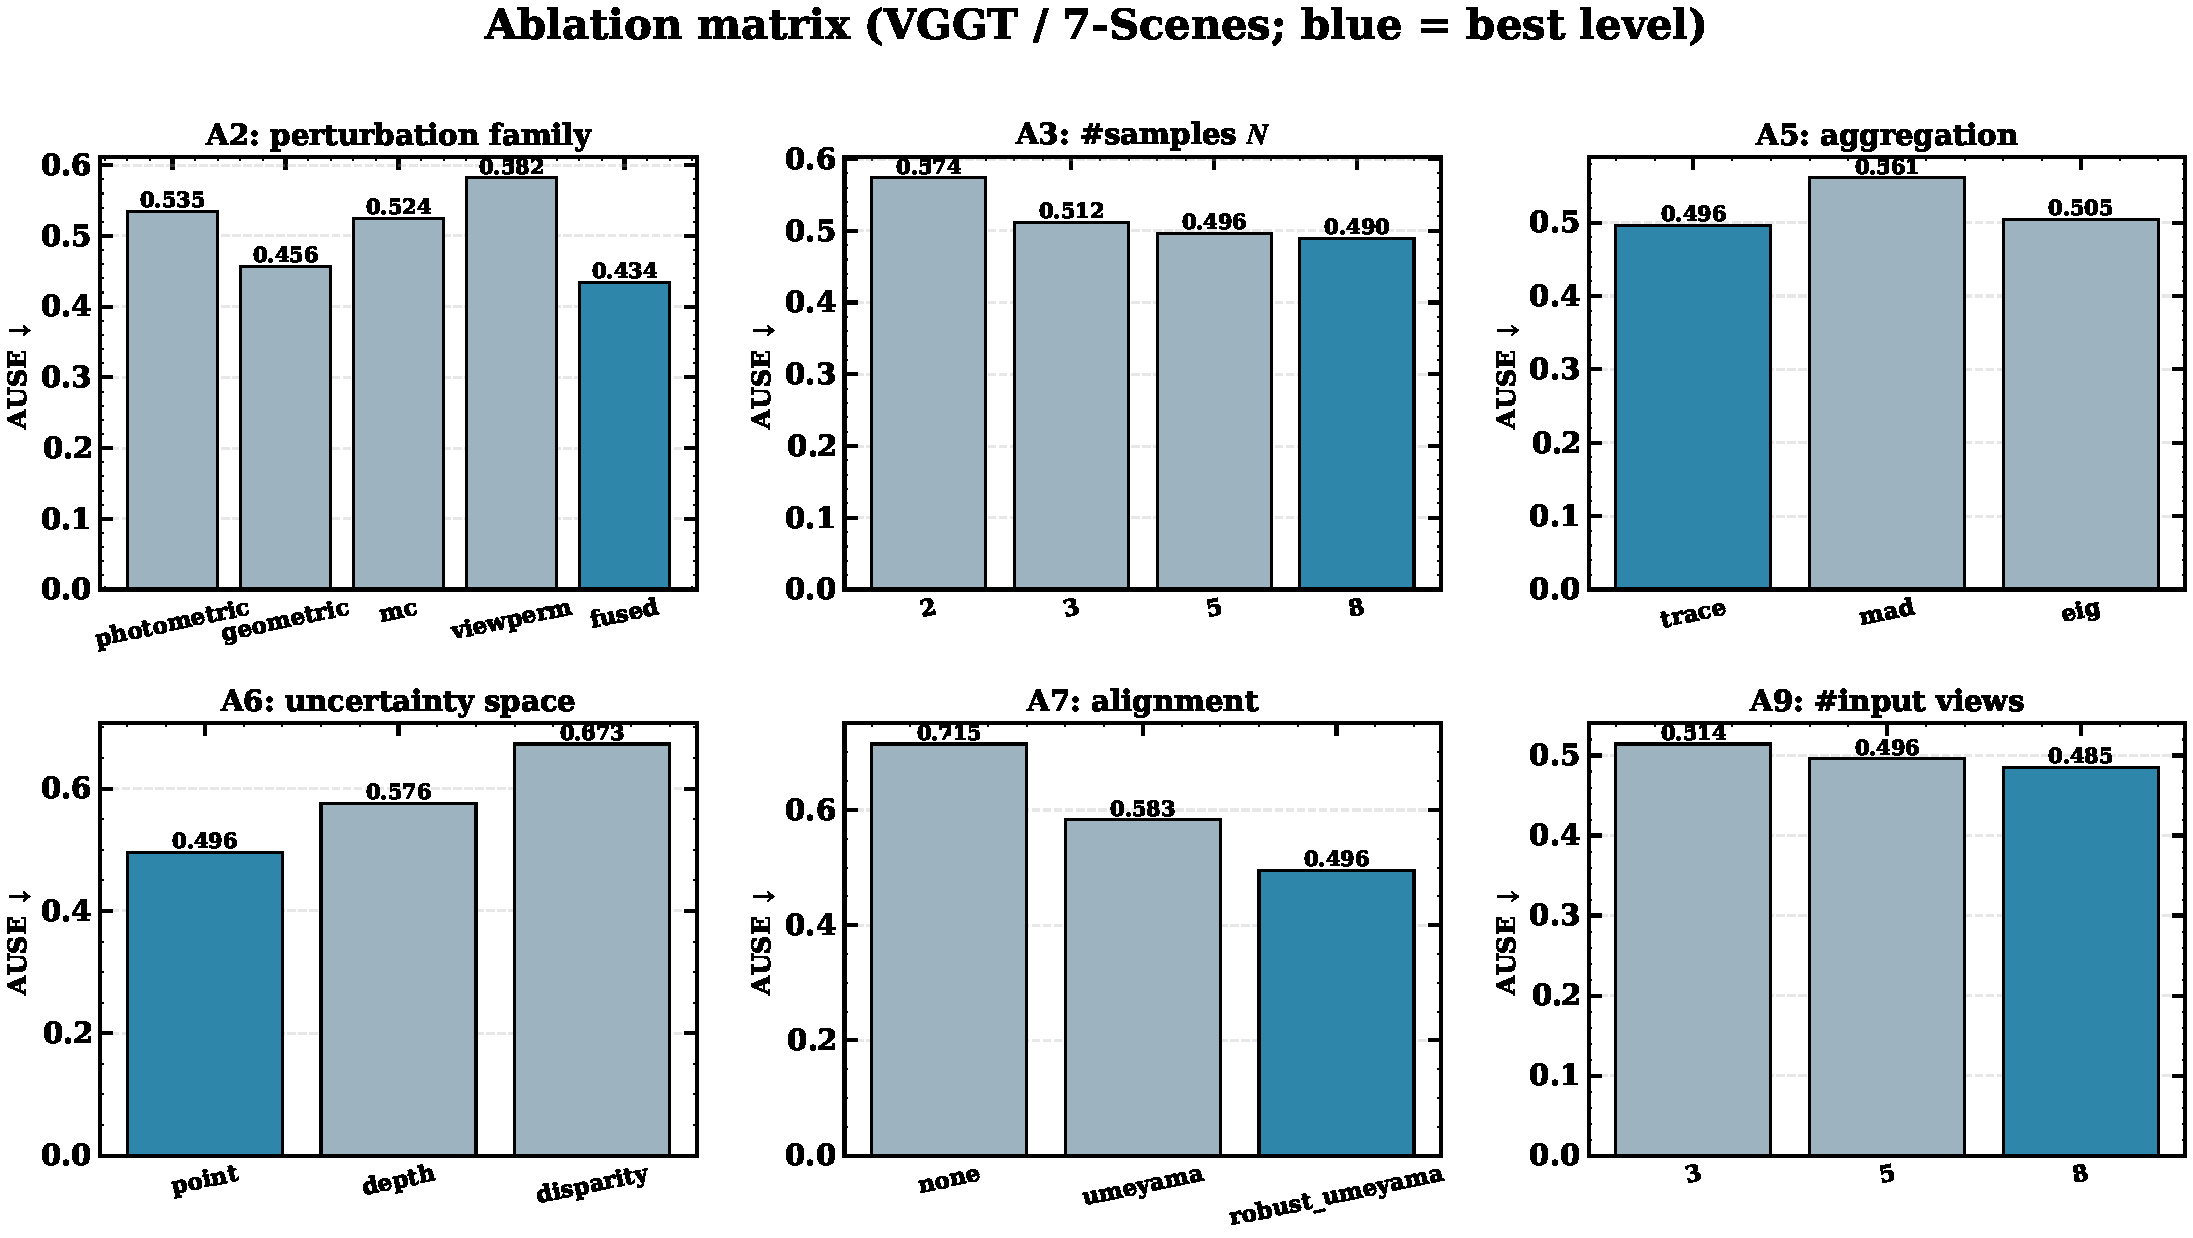
\includegraphics[width=0.95\textwidth]{ablation_grid.pdf}
  \caption{Ablation matrix (\vggt/7-Scenes; \ause\dn, blue $=$ best level per factor). Single-knob
  sweeps over perturbation family, sample count $N$, aggregation, uncertainty space, alignment, and
  input views.}
  \label{fig:ablgrid}
\end{figure*}

\subsection{The two design-defining knobs}
\label{sec:abl-standouts}

\paragraph{A7 --- alignment is the technical crux ($0.715\to0.583\to0.496$).} This is a $0.219$
absolute swing from worst to best---larger than any other knob, and larger than the gap between
\trustr\ and the built-in confidence itself. \emph{Why no alignment is near-random} ($0.715$): when
input views are permuted, \vggt/\mastr\ re-express the whole cloud in a different frame (rotation,
translation, \emph{and} global scale, since they lack metric scale). Without alignment the per-point
``spread'' is dominated by these \emph{common-mode} frame offsets---identical for every point---which
swamp the genuine, point-specific disagreement, giving an almost-flat, useless uncertainty.
\emph{Plain Umeyama} ($0.583$) removes the global offset, so the residual spread is mostly real
disagreement. \emph{Robust Umeyama} ($0.496$) additionally stops the worst-disagreeing
points---exactly the ones we want to flag---from tilting the fit and smearing their error onto the
good points. This row is the empirical content of the paper's central conceptual claim: in 3D the
runs live in incompatible frames, so alignment-before-variance is the method, not bookkeeping.

\paragraph{A8 --- calibration, measured in \ece\ not \ause\ ($0.296\to0.094$).} Calibration is a
monotone remap and \ause\ is rank-invariant, so calibration \emph{cannot} change \ause\ by
construction; measuring it in \ause\ would misleadingly show ``no effect.'' Its job is to make the
magnitude honest (a stated $90\%$ interval really contains $90\%$ of errors), scored by \ece, fit on
one half and evaluated on the held-out half. \emph{None} ($0.296$) is badly mis-calibrated.
\emph{Temperature} ($0.372$)---a single global multiplier---is \emph{worse than none}, because this
raw single-family uncertainty is mis-\emph{shaped}, not merely mis-\emph{scaled}, and one scalar
cannot fix a nonlinear distortion. \emph{Isotonic} ($0.094$)---an arbitrary monotone
Pool-Adjacent-Violators curve---matches the shape of the error distribution and cuts \ece\ roughly
$3\times$ while preserving ranks (hence \ause).

\subsection{The remaining knobs, briefly}
\label{sec:abl-rest}

\begin{itemize}[leftmargin=1.4em,itemsep=2pt,topsep=2pt]
\item \textbf{A1 (base model).} \trustr\ generalizes: \vggt\ $0.496$ and \pii\ $0.380$, both far below
their built-in baselines ($0.710$ and $0.509$). \pii's lower absolute \ause\ is an easier base signal,
not a \vggt\ failure.
\item \textbf{A2 (perturbation family).} photo $0.535$, geom $0.456$, mc $0.524$, viewperm $0.582$,
\emph{fused} $0.434$: the fusion beats every single family---no one perturbation is best.
\item \textbf{A3 (samples $N$).} $0.574/0.512/0.496/0.490$ for $N{=}2/3/5/8$: a sharp gain to $N{=}5$,
then flat ($5\to8$ moves \ause\ by $0.0006$). $N{=}5$ is the cost/quality knee; $N{=}3$ already
recovers $\approx 93\%$ of the gain.
\item \textbf{A4 (photometric strength).} $0.532/0.535/0.543$ for low/med/high: a spread of $\approx
0.01$---essentially insensitive, so the recipe is not a tuned hyper-parameter.
\item \textbf{A5 (aggregator).} trace $0.496$, MAD $0.561$, eig $0.505$: trace-variance is best.
\item \textbf{A6 (uncertainty space).} point $0.496$, depth $0.576$, disparity $0.673$: measuring
spread in native 3D-point space is materially better than in depth or disparity.
\item \textbf{A9 (input views).} $0.514/0.496/0.485$ for $3/5/8$ views: more views help with
diminishing returns; $5$ is the default knee.
\item \textbf{A11 (view-perm mode).} shuffle $0.582$ vs.\ subset $0.581$: a tie on the
reference-dependent \vggt\ (both expose reference instability). For the equivariant \pii, shuffle is
inert and subset is the one that works (\Cref{sec:exp-arch}).
\item \textbf{A12 (fusion weighting).} equal $0.586$ vs.\ learned $0.585$: close in-distribution; the
value of the held-out weighting shows up against the built-in baseline once it is a fusion family
(\Cref{sec:abl-fusion}).
\item \textbf{A13/A14 (downstream).} the 3DGS-initialization null and the multi-view-fusion win,
already reported in \Cref{sec:exp-fusion,sec:exp-neg}.
\end{itemize}

\subsection{Calibration generalizes across the grid, and needs almost no ground truth}
\label{sec:abl-calib}

\Cref{fig:reliability} (A8) is the raw single-family signal on one cell. \Cref{tab:q2ece} reports the
regression \ece\ of the \emph{headline fused} signal for all twelve cells, before and after the
isotonic step (held-out 2-fold over view-sets). With a single global scale the fused signal is already
moderately calibrated (\ece\ $0.04$--$0.15$); the isotonic map reduces \ece\ further where it is
largest---the out-of-distribution ETH3D cells (e.g.\ \pii/ETH3D $0.072\to0.037$) and the higher-error
DTU cells (\mastr/DTU $0.146\to0.103$)---and is approximately neutral on the already-low cells.

\begin{figure}[tb]
  \centering
  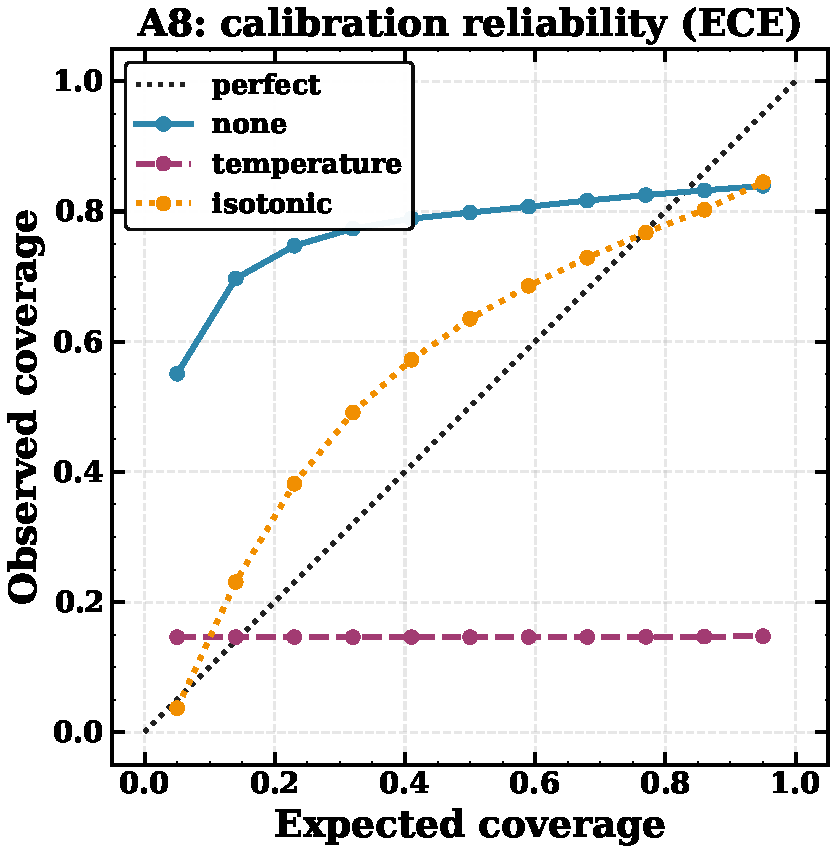
\includegraphics[width=0.8\linewidth]{A8_reliability.pdf}
  \caption{Calibration reliability (A8): the isotonic mapping brings observed coverage onto the
  diagonal, cutting \ece\ $\sim 3\times$.}
  \label{fig:reliability}
\end{figure}

\begin{table*}[tb]
\centering\small
\adjustbox{max width=\textwidth}{\input{tables/tab_q2_ece}}
\caption{Per-cell regression \ece\dn\ of the headline fused signal: a single global scale (``raw'')
vs.\ a held-out isotonic map. Isotonic helps most on the out-of-distribution and higher-error cells.}
\label{tab:q2ece}
\end{table*}

How much ground truth does calibration actually need? \Cref{tab:q6} answers directly. The registered
cross-run spread is a faithful \emph{rank} predictor of error---all \ause\ and the fusion use---but it
systematically \emph{under}-estimates the absolute error (it measures epistemic input-sensitivity,
not total error), so used as a raw $\sigma$ it is maximally mis-calibrated (\ece\ $\approx 0.50$). A
\emph{single} global scale, estimable from any small labelled sample, removes this bias and recovers
most of the calibration (\ece\ $0.50\to0.14$ on average); a small held-out isotonic split refines it
to $0.08$. The method's ground-truth requirement thus reduces to \emph{one scalar} for absolute
coverage---the ranking, \ause, and fusion are entirely ground-truth-free.

\begin{table*}[tb]
\centering\small
\adjustbox{max width=\textwidth}{\input{tables/tab_q6_calib}}
\caption{\textbf{Calibration needs only one scalar of ground truth.} Regression \ece\dn\ of the metric
perturbation uncertainty under three calibrations: raw $\sigma$ (no GT), a single global scale (one
number of GT), and a held-out isotonic map. One scalar removes the systematic under-confidence.}
\label{tab:q6}
\end{table*}

\subsection{Fusion: equal vs.\ held-out weighting, and is the headline circular?}
\label{sec:abl-fusion}

\Cref{tab:allsig} reports \ause\ for \emph{every} signal across all twelve cells---the built-in
confidence, the MC baseline, the two standalone \trustr\ families, and the two fusions. Two patterns underpin the main
text. First, view-permutation is the strongest single family on the reference-dependent \vggt/\mastr\
and weaker (though not inert) on \pii, where its signal comes from leave-one-out subset rather than
shuffle. Second, the held-out weighted fusion and the equal-weight fusion are close but not identical.

\begin{table*}[tb]
\centering\small
\adjustbox{max width=\textwidth}{\input{tables/tab_allsignals}}
\caption{Per-signal \ause\dn\ (mean over 3 seeds) for all 12 cells. Columns: built-in confidence;
MC/latent-noise baseline; the two standalone \trustr\ families (photometric, view-perm); and the
equal-weight and held-out-weighted fusions. \best{Bold} marks the best (lowest) signal in each row.}
\label{tab:allsig}
\end{table*}

\paragraph{Equal vs.\ held-out weighting.} \Cref{tab:fuserob} contrasts the two directly. Against the
built-in baseline, the held-out weighting wins $9$ of $12$ cells to equal fusion's $8$; crucially it
\emph{recovers} \pii/DTU---the one cell the perturbation families alone regress---which equal fusion
turns into a regression. Equal fusion is, in turn, marginally stronger on the out-of-distribution
ETH3D cells, where admitting the correlation-collapsed built-in confidence as a candidate slightly
dilutes the perturbation signal. The mechanism is structural: under shift the built-in confidence is
collapsed in rank correlation ($\rho\approx 0$) yet only \emph{moderately} worse in \ause\ than the
perturbation families, and because the inverse-\ause\ weight is soft it cannot drive a moderately-worse
family to zero---so the collapsed built-in still earns roughly a fifth to a quarter of the weight and
dilutes the cleaner perturbation signal. Two facts keep this in perspective: \emph{(i)} both fusions
still beat the built-in confidence on every OOD cell, so the headline OOD result is invariant to the
fusion choice; and \emph{(ii)} the weighting earns its keep in-distribution (the \pii/DTU recovery)
and never collapses far below a genuinely-good confidence. We therefore adopt the held-out weighting
as the principled, leakage-free default, and note that under \emph{known} domain shift the simpler
choice---drop the built-in family and use a perturbation-only fusion---is marginally better.

\begin{table*}[tb]
\centering\small
\adjustbox{max width=\textwidth}{%
\begin{tabular}{llcc}
\toprule
Model & Dataset & Equal fusion & \trustr\ (held-out $+$ built-in) \\
\midrule
\vggt & 7-Scenes & 0.537 & 0.492 \\
\vggt & DTU & 0.198 & 0.175 \\
\vggt & ETH3D (OOD) & 0.610 & 0.673 \\
\vggt & BlendedMVS & 0.286 & 0.405 \\
\pii & 7-Scenes & 0.351 & 0.359 \\
\pii & DTU & 0.340 & 0.231 \\
\pii & ETH3D (OOD) & 0.480 & 0.616 \\
\pii & BlendedMVS & 0.234 & 0.281 \\
\mastr & 7-Scenes & 0.404 & 0.354 \\
\mastr & DTU & 0.320 & 0.352 \\
\mastr & ETH3D (OOD) & 0.600 & 0.644 \\
\mastr & BlendedMVS & 0.377 & 0.308 \\
\bottomrule
\end{tabular}}
\caption{Equal vs.\ held-out weighted fusion (\ause\dn, mean over 3 seeds). The held-out weighting
adds the built-in confidence as a fusion family: it wins more cells against the built-in baseline
($9$ vs.\ $8$) and recovers \pii/DTU, while equal fusion is marginally stronger OOD.}
\label{tab:fuserob}
\end{table*}

\paragraph{Is the comparison circular?} Including the built-in confidence as a fusion family invites
the worry that beating that same confidence is rigged. It is not. \Cref{tab:q3decouple} removes the
built-in family from the fusion entirely: a held-out, inverse-\ause\ rank fusion of the two
\emph{perturbation} families alone still significantly beats the built-in confidence on $8$ of $12$
cells. Re-adding the built-in family as a third candidate lifts this to $9/12$, the single additional
cell being \pii/DTU. The training-free perturbation signal therefore carries the result on its own;
the built-in family helps only where it is genuinely informative, and the three non-wins are exactly
the BlendedMVS column, the models' own training corpus.

\begin{table*}[tb]
\centering\small
\adjustbox{max width=\textwidth}{\input{tables/tab_q3_fusion}}
\caption{\textbf{Decoupling the headline from the baseline} (\ause\dn, held-out fusion, mean over 3
seeds). \best{Bold} marks a significant per-set win over the built-in confidence. Perturbation-only
fusion (\emph{no} built-in) already wins $8/12$; adding the built-in family reaches $9/12$, recovering
\pii/DTU. The three non-wins are exactly the BlendedMVS training corpus.}
\label{tab:q3decouple}
\end{table*}
